% $Id%

% ++++++++++++++++++++++++++++++++++++++++++++++++++++++++++++++++++++++++++
\newpage
\hypertarget{appendix-start}{}\label{s:appendix-start}

\section{Appendix}

    \begin{itemize}

      \item[1] \hyperlink{appendix-menutree}{CrypTool Menu Tree}

      \item[2] \hyperlink{appendix-authors}{Authors of the CrypTool Script}

      \item[3] \hyperlink{appendix-authors}{Bibliography of Movies and
                     Fictional Literature with Relation to Cryptograpy,
                     Books for Kids with Collections of Simple Ciphers}

      \item[4] \hyperlink{appendix-Learn-NT}
                     {Learning Tool for Elementary Number Theory}

    \end{itemize}




% ++++++++++++++++++++++++++++++++++++++++++++++++++++++++++++++++++++++++++
%\pagebreak
\newpage
\enlargethispage{1cm}
\hypertarget{appendix-menutree}{}
\subsection{CrypTool Menus}
\label{s:appendix-menutree}

This appendix contains at the following page the complete menu tree of
CrypTool\index{CrypTool} version 1.4.10. 

Which menu items in CrypTool are active (that means not greyed), depends on
the type of the currently active document window.

The brute-force analysis\index{Attack!brute-force} for DES e.~g. is only
available, if the active window is opened in the hexadecimal view. 
On the other hand the menu item ``Generate Random Numbers\dots''
is always available (even if no document is opened).

%The following four types of documents exist in CrypTool:
%\begin{center}
%\begin{tabular}{rl}
%\bf Code letter & \bf Type of document \\
%T & Text file view\\
%H & Hexadecimal view\\
%P & Diagram/plot view (histogram, autocorrelation)\\
%O & OpenGL graphics view\\
%\end{tabular}
%\end{center}


%\nobreak
\clearpage
\begin{figure}[hb]
\begin{center}
\vspace{-30pt}
%\frame{  %TeX macht einen Rehmen (siehe viewport) drumherum -- gut zum Testen
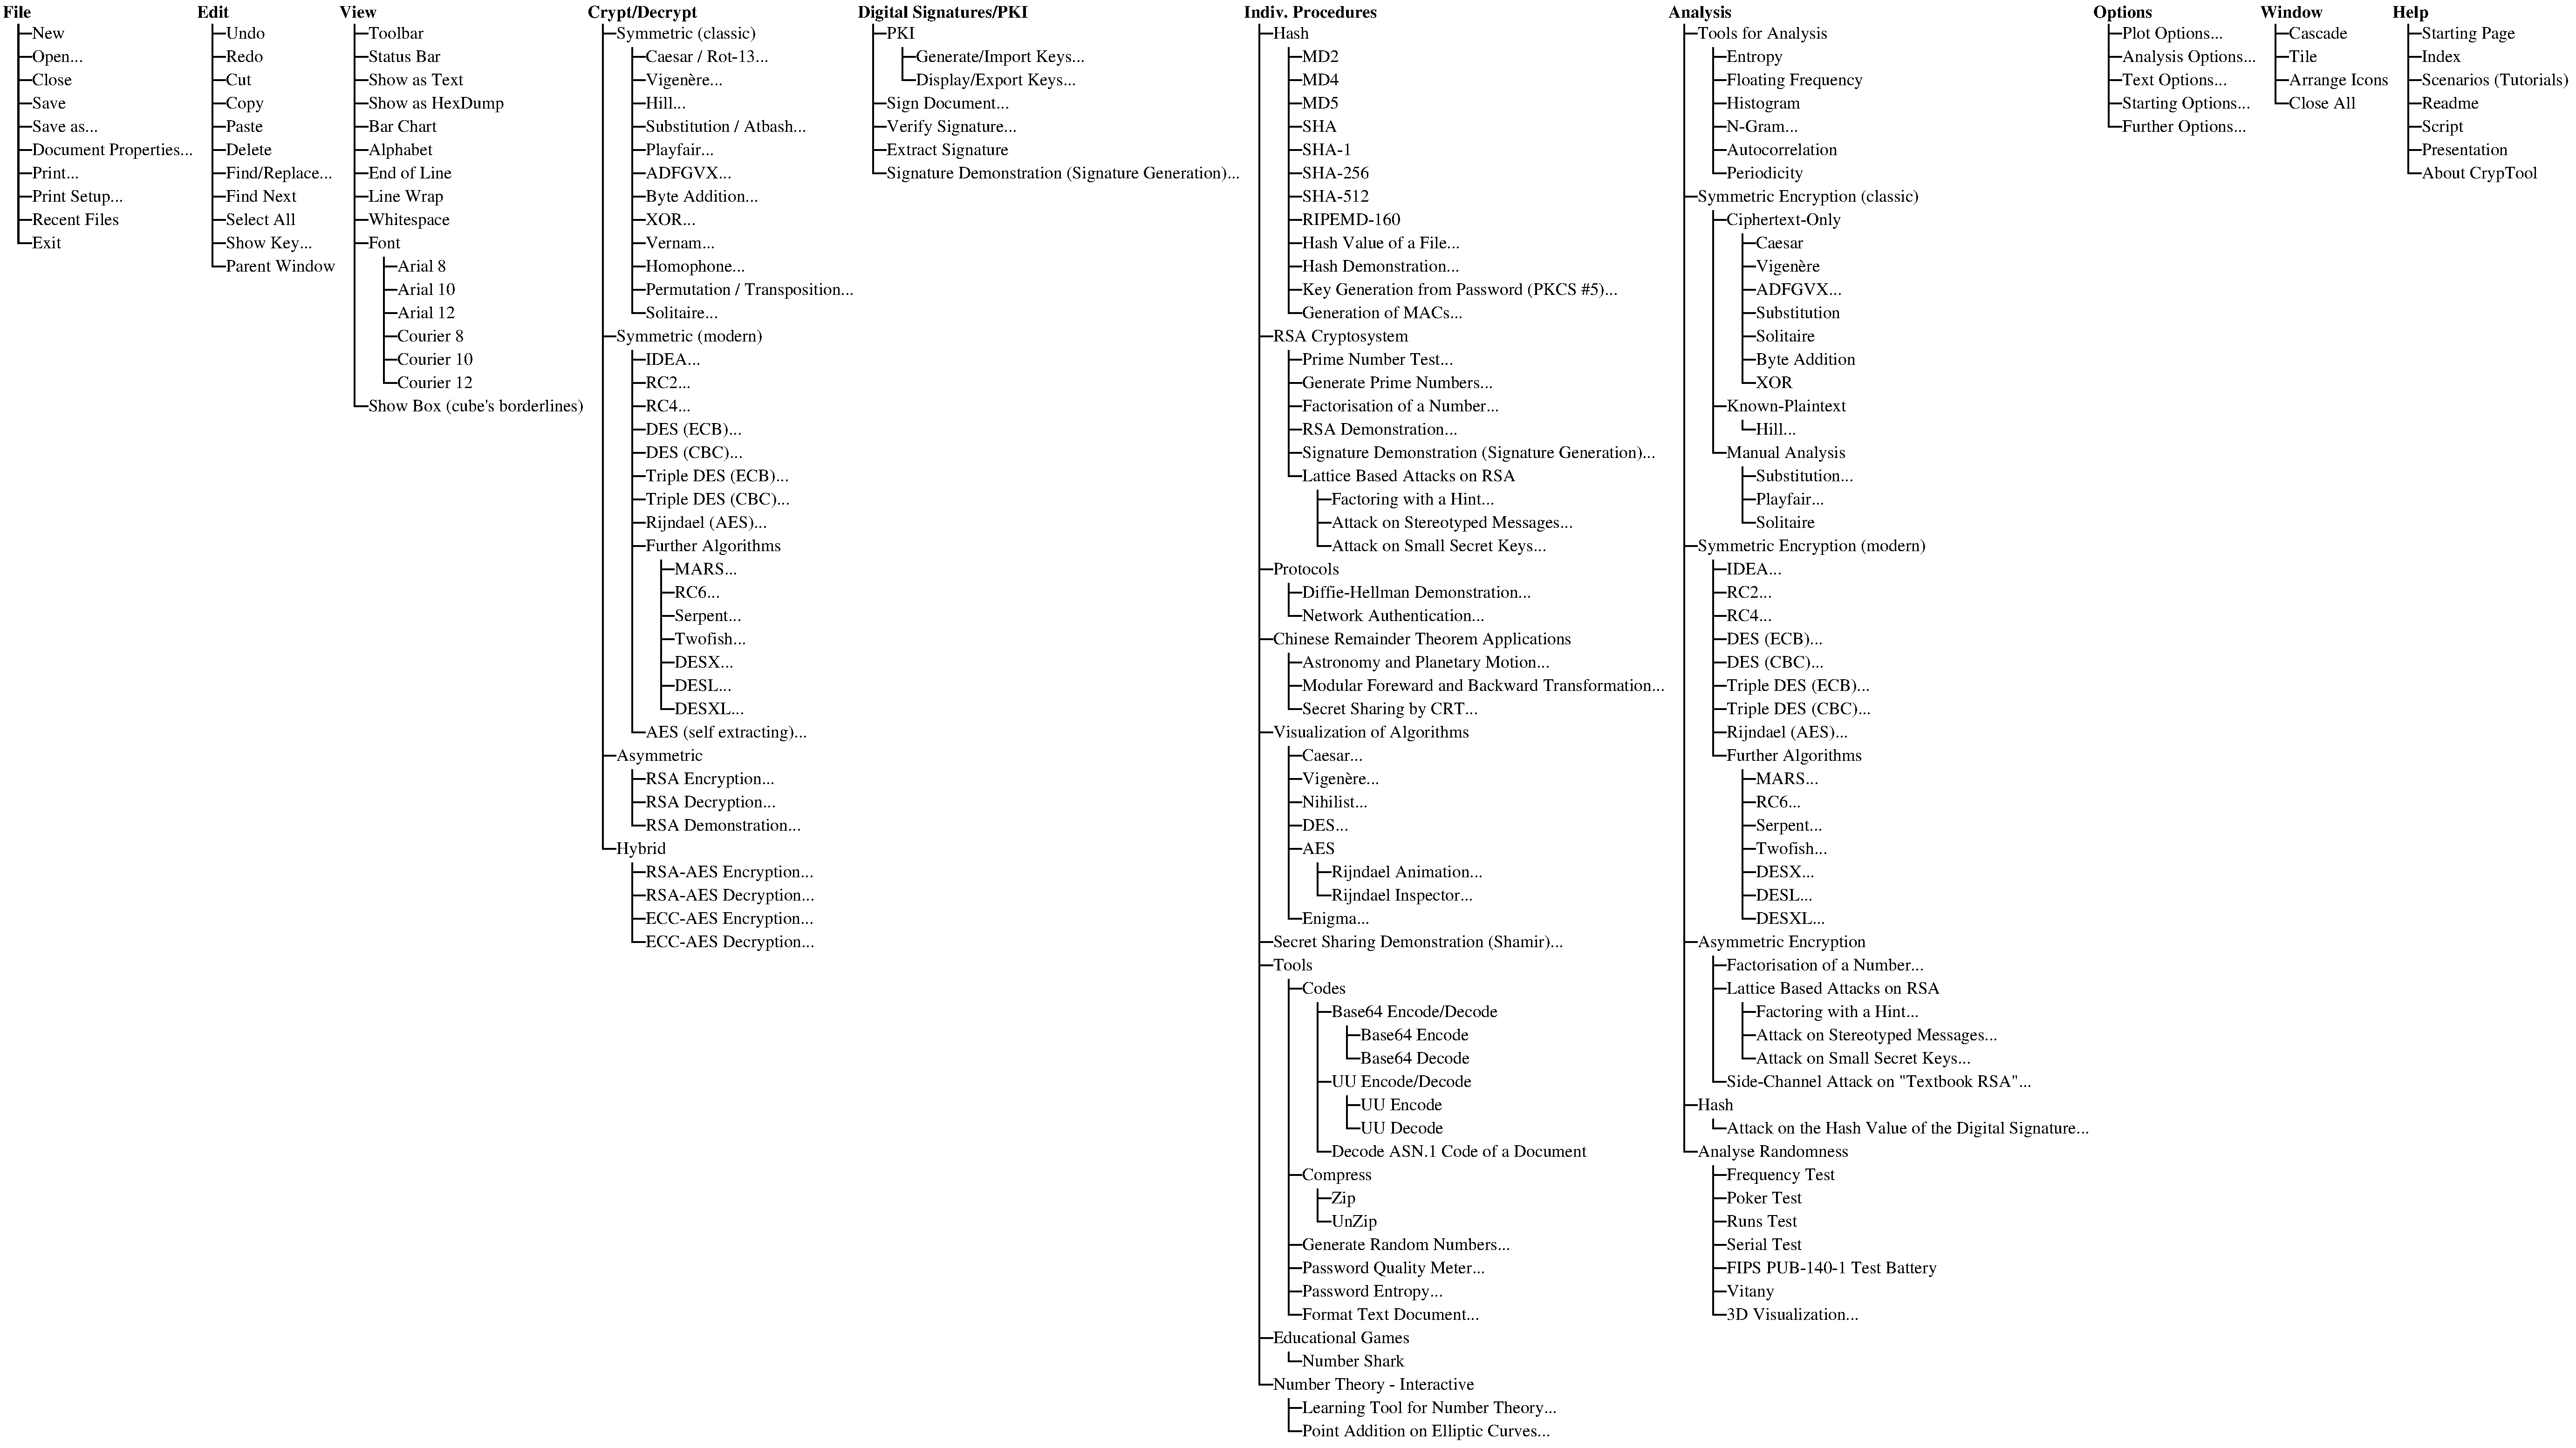
\includegraphics[scale=0.25, angle=270, viewport=200 30 2660 1430]
                {figures/cryptool-menu-en}
%viewport=rand-links? rand-unten breite hoehe? [bezogen auf querformat]
%}
\caption{Complete overview of the menu tree of CrypTool 1.4.20} 
\label{menuoverview}
\end{center}
\end{figure}
\clearpage

